\documentclass[11pt,a4paper]{beamer}

\usepackage[utf8]{inputenc}
\usepackage[english]{babel}
\usepackage[T1]{fontenc}
\usepackage{amsmath}
\usepackage{amsfonts}
\usepackage{amssymb}
\usepackage{graphicx}
\usepackage{bbm}
\usepackage{ulem}
\usepackage{color}
\usepackage{tikz}
%\usepackage{pdfpages}

\usetheme{Boadilla} %+ color default
%\usetheme{default}
%\useoutertheme{bapt}


\definecolor{slineColor}{RGB}{81,22,97}


\setbeamertemplate{footline}
{
  \leavevmode%
  \hbox{%
  \begin{beamercolorbox}[wd=.25\paperwidth,ht=2.25ex,dp=1ex,center]{author in head/foot}%
    \usebeamerfont{author in head/foot}\insertshortauthor
  \end{beamercolorbox}%
  \begin{beamercolorbox}[wd=.50\paperwidth,ht=2.25ex,dp=1ex,center]{title in head/foot}%
    \usebeamerfont{title in head/foot}\insertshorttitle
  \end{beamercolorbox}%
  \begin{beamercolorbox}[wd=.25\paperwidth,ht=2.25ex,dp=1ex,right]{date in head/foot}%
    \usebeamerfont{date in head/foot}\insertshortdate{}\hspace*{2em}
    \insertframenumber{} / \inserttotalframenumber\hspace*{2ex} 
  \end{beamercolorbox}}
  \vskip0pt%
}
\setbeamertemplate{blocks}[rounded][shadow=true]
%\setbeamertemplate{frametitle}[horizontal shading]{left=slineColor, right=white}
%\setbeamertemplate{frametitle}
%{
%    \begin{beamercolorbox}[ht=1.8em,wd=\paperwidth]{frametitle}
%        \insertframetitle
%    \end{beamercolorbox}
%}






%%%%
%%%% BLOCK COLORS
%%%%

\setbeamercolor{block title}{fg=black,bg=blue!50}
\setbeamercolor{block body}{fg=black,bg=blue!10}
%\setbeamercolor{block title}{fg=black,bg=slineColor!60}

\setbeamercolor{block title alerted}{fg=black,bg=red!80}
\setbeamercolor{block body alerted}{fg=black,bg=red!10}


%\setbeamercolor{author in head/foot}{bg=slineColor}
%\setbeamercolor{title in head/foot}{bg=slineColor!80}
%\setbeamercolor{date in head/foot}{bg=slineColor!60}

%\setbeamercolor{frametitle}{bg=slineColor!80, fg=white}
%\setbeamercolor{frametitle}{fg=slineColor!80}

%\setbeamercolor{title}{fg=slineColor!80}
%\setbeamercolor{section in toc}{fg=slineColor!80}

%%%%
%%%% CONTENTS
%%%%

%\AtBeginSection[]{
%	\AtBeginSubsection[]{
%		\begin{frame}
%			\begin{flushleft}{\Large Contents }\end{flushleft}
%			\tableofcontents[currentsection, currentsubsection]
%		\end{frame} 
%	}
%}
%

\AtBeginSection[]{
%	\AtBeginSubsection[]{
		\begin{frame}
			\begin{flushleft}{\Large Plan }\end{flushleft}
			\tableofcontents[currentsection, hideallsubsections]
		\end{frame} 
%	}
}



%%%%
%%%% LOGOS ET IMAGES
%%%%

%\pgfdeclareimage[height=0.85cm]{logo-gauche}{/mon/logo/nom_sans_point_ps}
%\pgfdeclareimage[height=0.85cm]{logo-droite}{/chemin/de/mon/second/logo}
%\logo{\pgfuseimage{logo-droite}}
%
%\setbeamertemplate{sidebar left}
%{
%\logo{\pgfuseimage{logo-gauche}}
%\vfill%
%\rlap{\hskip0.1cm\insertlogo}%
%\vskip15pt%
%}

%\logo{\includegraphics[height=8mm]{C:/Users/LSTA/Documents/LateX/includes/sline.png}}
%\titlegraphic{\includegraphics[height=8mm]{C:/Users/LSTA/Documents/LateX/includes/sline.png}}
%\hspace{280pt}

 

\DeclareMathOperator*{\Argmin}{arg\,min}
\newcommand{\argmin}[1]{\Argmin\limits_{#1}}
\usepackage{hyperref}


\usepackage{listings}
\usepackage{xcolor}

\definecolor{codegreen}{rgb}{0,0.6,0}
\definecolor{codegray}{rgb}{0.5,0.5,0.5}
\definecolor{codepurple}{rgb}{0.58,0,0.82}
\definecolor{backcolour}{rgb}{0.95,0.95,0.92}

\lstdefinestyle{mystyle}{
    backgroundcolor=\color{backcolour},   
    commentstyle=\color{codegreen},
    keywordstyle=\color{magenta},
    numberstyle=\tiny\color{codegray},
    stringstyle=\color{codepurple},
    basicstyle=\ttfamily\footnotesize,
    breakatwhitespace=false,         
    breaklines=true,                 
    captionpos=b,                    
    keepspaces=true,                 
    numbers=left,                    
    numbersep=5pt,                  
    showspaces=false,                
    showstringspaces=false,
    showtabs=false,                  
    tabsize=2
}

\lstset{style=mystyle}



\title[Autoencoder]{An introduction to Autoencoders}
\author{Baptiste Gregorutti}



\begin{document}

\begin{frame}
\bigskip
\maketitle
\end{frame}

\begin{frame}
	\frametitle{Autoencoders Content}

	\begin{itemize}
		\item Mathematical definitions
		\item Relations with the PCA (linear transformation) : AE performs a nonlinear transformation through a nonlinear activation function (e.g. ReLu, sigmoid)
		\item types of AE: MLP, Deep MLP, Convolutional, Recurrent
		\item applications to autoencoders
	\end{itemize}

\end{frame}




\begin{frame}
	\frametitle{Definition}

	\begin{block}{}
	Autoencoders are a type of self-supervised learning model that can learn a \textbf{compressed representation} of input data.
	\end{block}

	\bigskip
	\centering
	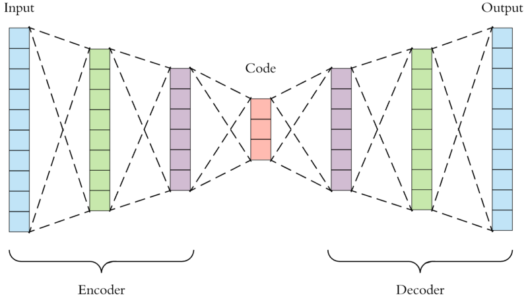
\includegraphics[width = 0.6\textwidth]{figures/AE.png}

\end{frame}



\begin{frame}
	\frametitle{Definition}

	\begin{block}{}
	Let $\mathcal X$ be the original space and $\mathcal F$ be a latent space.
	\begin{itemize}
		\item Encoding function $\phi : \mathcal X \longrightarrow \mathcal F$
		\item Decoding function $\psi : \mathcal F \longrightarrow \mathcal X$
	\end{itemize}
	We have to find the optimal encoding and decoding function by minimizing
	$$\phi^\star, \psi^\star \in \argmin{\phi, \psi} \left\Vert X - (\psi \circ \phi) X \right\Vert^2$$
	\end{block}

	Two networks:
	\begin{itemize}
		\item Encoding network $\mathbf z = \sigma(\mathbf W \mathbf x + \mathbf b)$
		\item Decoding network $\mathbf x' = \sigma(\mathbf W' \mathbf z + \mathbf b')$
		\item Loss function: $\mathcal L(\mathbf x, \mathbf x') = \left\Vert \mathbf x - \mathbf x' \right\Vert^2$
	\end{itemize}
	
\end{frame}


\begin{frame}
	\frametitle{Hyperparameters of autoencoders}
	There are 5 hyperparameters:
	\begin{itemize}
		\item Dimension of the latent space
		\item Activation function
		\item Number of layers
		\item Number of nodes per layers
		\item Loss function
	\end{itemize}
\end{frame}


\begin{frame}[containsverbatim]
	\frametitle{In practice ?}

	\begin{lstlisting}[language=Python]
		input_img = Input(input_dim)
		encoded = Dense(lat_dim, activation='relu')(input_img)
		decoded = Dense(inp_dim, activation='sigmoid')(encoded)
		autoencoder = Model(input_img, decoded)
	\end{lstlisting}
\end{frame}


\begin{frame}
	\frametitle{Relationships with the Principal Components Analysis}

	\begin{block}{}
		An autoencoder with a \textbf{single fully-connected hidden layer}, a \textbf{linear activation function} and a \textbf{squared error cost function} trains weights that span the same subspace as the one spanned by the principal component loading vectors
	\end{block}

	\centering
	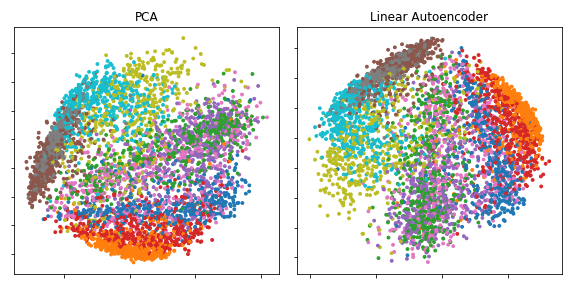
\includegraphics[width=0.6\textwidth]{figures/PCA_vs_Linear_Autoencoder.png}

\end{frame}

\begin{frame}
	\frametitle{Deep autoencoders}
	\centering
	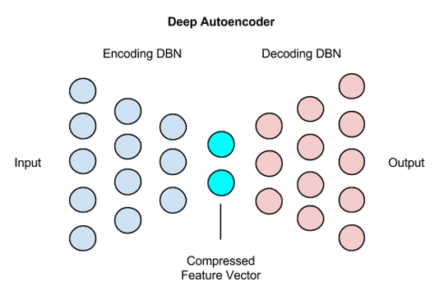
\includegraphics[width=0.8\textwidth]{figures/deep_AE.png}
\end{frame}

\begin{frame}
	\frametitle{Convolutional autoencoders}
	\centering
	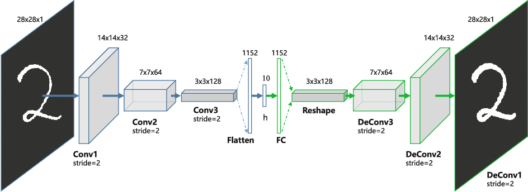
\includegraphics[width=0.8\textwidth]{figures/CNN_AE.png}
\end{frame}

\begin{frame}
	\frametitle{Recurrent autoencoders}
	\centering
	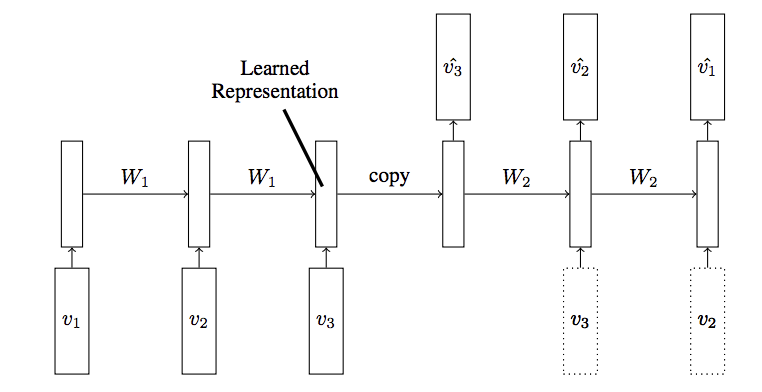
\includegraphics[width=0.8\textwidth]{figures/LSTM_AE.png}
\end{frame}



\begin{frame}
	\frametitle{Applications to autoencoders}

	Applications:
	\begin{itemize}
		\item Data compression
		\item Image reconstruction
		\item Image colorization
		\item Denoising
	\end{itemize}

\end{frame}




\begin{frame}
	\frametitle{Take away message}

	\begin{itemize}
		\item An autoencoder can learn non-linear transformations with a non-linear activation function and multiple layers
		\item It doesn’t have to learn dense layers. It can use convolutional layers to learn which is better for video, image and series data.
		\item It is more efficient to learn several layers with an autoencoder rather than learn one huge transformation with PCA.
	\end{itemize}

\end{frame}




\begin{frame}
	\frametitle{Variational autoencoders}

	\begin{block}{Idea}
		A variational autoencoders is a \textbf{generative model}, mainly used for content generation (images, sounds, etc.)
	\end{block}

	\centering
	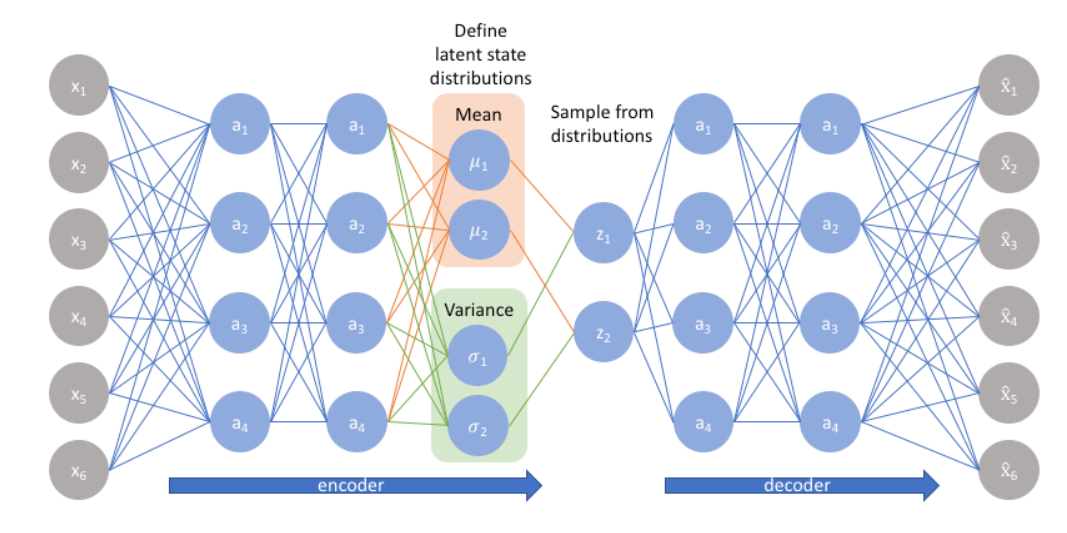
\includegraphics[width=0.8\textwidth]{figures/VAE.png}

\end{frame}





\begin{frame}
	\frametitle{References}
	\begin{itemize}
		\item \href{https://blog.keras.io/building-autoencoders-in-keras.html}{Keras blog}  
		\item \href{https://towardsdatascience.com/generating-images-with-autoencoders-77fd3a8dd368}{Comprehensive Introduction to Autoencoders, Matthew Stewart}
		\item \href{https://medium.com/edureka/autoencoders-tutorial-cfdcebdefe37}{How To Perform Data Compression Using Autoencoders?, Sayantini Deb}
		\item \href{https://machinelearningmastery.com/lstm-autoencoders/}{A Gentle Introduction to LSTM Autoencoders, Jason Brownlee}
		\item \href{hhttps://towardsdatascience.com/understanding-variational-autoencoders-vaes-f70510919f73}{Understanding Variational Autoencoders, Joseph Rocca}
	\end{itemize}
\end{frame}


\end{document}


